
% vim:set ff=unix expandtab ts=2 sw=2:
%\begin{multicols}{2}
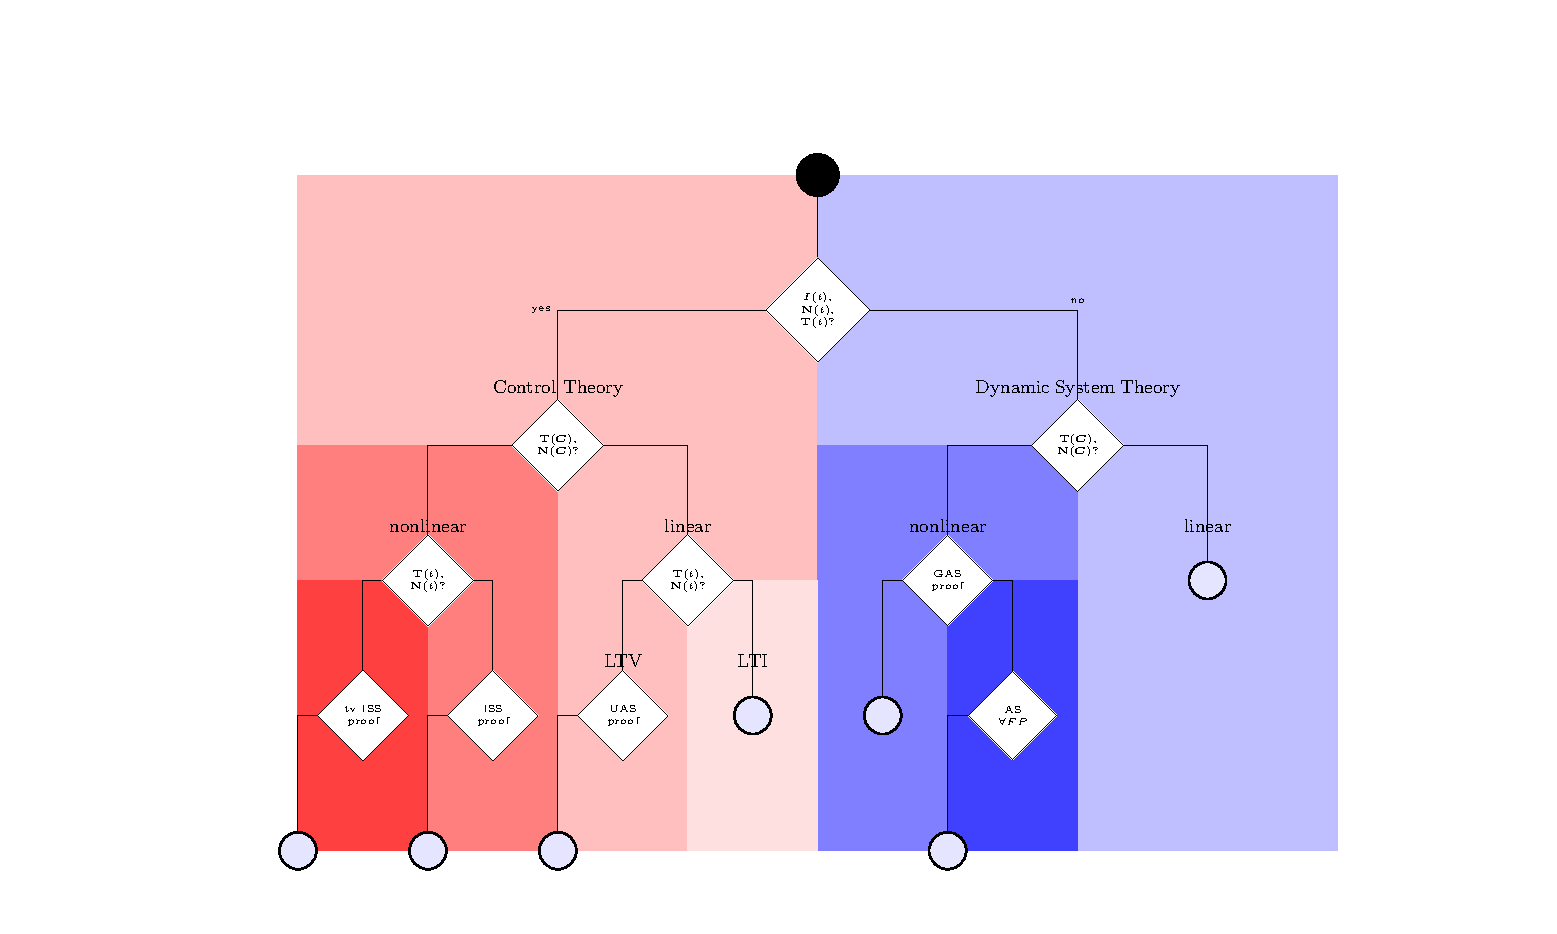
\includegraphics[width=\columnwidth,clip=true,trim=4.5cm 1cm 1cm 1cm]{Fig1.pdf}

%\columnbreak
\noindent
The graph shows different stability concepts one could try to establish for the
general soil model mentioned above depending on properties of its components 
$\mathbf{I},\mathbf{T}$ and $ \mathbf{N}$. The hardest to prove is Input to
State Stability for time varying systems (ISStv) in the lower left corner.  It
turns out that ISStv also generalizes all the other concepts mentioned:
\begin{itemize}
\item 
In the case of Linear Time Invariant (LTI) systems  ISS follows from the properties of the matrix.(eigenvalues)
\item 
In the case of Linear Time Variant (LTV) systems it can be established if sufficient information about the 
state transition operator allows to prove uniform asymptotic stability UAS.
\item
For input free system (on the blue right-hand side) ISS reduces to Global Asymptotic Stability (GAS)
\item
\dots

\end{itemize}
%\end{multicols}
